% Import default values & document settings
% Layout settings
\newcommand{\FIITdefaultFontSize}[0] {12pt}
\setcounter{secnumdepth}{3}
\setcounter{tocdepth}{3}

% Language settings
\newcommand{\FIITlanguage}[0] {slovak}
% \newcommand{\FIITlanguage}[0] {slovak,english}
%\def\FIITlagEN{}

% Global texts
\newcommand{\FIITuniversity}[0] {Slovak University of Technology in Bratislava}
\newcommand{\FIITuniversitySK}[0] {Slovenská technická univerzita v Bratislave}
\newcommand{\FIITfaculty}[0] {Faculty of informatics and information technologies}
\newcommand{\FIITfacultySK}[0] {Fakulta informatiky a informačných technológií}
\newcommand{\FIITthesis}[0] {Bachelor's thesis}
\newcommand{\FIITthesisSK}[0] {Bakalárska práca}
\newcommand{\FIITtitle}[0] {Research in the field of Digital Twin technology}
\newcommand{\FIITtitleSK}[0] {Výskum v oblasti technológie digitálneho dvojčaťa}
\newcommand{\FIITauthor}[0] {Dávid Truhlář}
\newcommand{\FIITsupervisor}[0] {Ing. Matej Petrík}
\newcommand{\FIITevidenceNumber}[0] {FIIT-16768-120897}
\newcommand{\FIITdate}[0] {May 2025}
\newcommand{\FIITdateSK}[0] {Máj 2025}
\newcommand{\FIITstudyProgram}[0] {Informatics}
\newcommand{\FIITstudyProgramSK}[0] {Informatika}
\newcommand{\FIITstudyField}[0] {Computer Science}
\newcommand{\FIITdegreeCourseSK}[0] {Informatika}
\newcommand{\FIITinstitute}[0] {Institute of Computer Engineering and Applied Informatics}
\newcommand{\FIITinstituteSK}[0] {Ústav počítačového inžinierstva a aplikovanej informatiky}
\newcommand{\FIITsignPlace}[0] {In Bratislava, }
\newcommand{\FIITsignPlaceSK}[0] {V Bratislave, }
\newcommand{\FIITsignDate}[0] {12.5.2025}
\newcommand{\FIITArchiveName}[0] {BP\_prilohy\_digital\_JanoMrkvicka.zip}


% Setup document
\documentclass[\FIITdefaultFontSize,a4paper,twoside,openright,\FIITlanguage]{book}

% Load all necessary packages
\usepackage[final]{pdfpages}
\usepackage[utf8]{inputenc}
\usepackage[T1]{fontenc}
\usepackage[\FIITlanguage]{babel}
\usepackage[a4paper]{geometry}
\usepackage[
    left = \glqq,% 
    right = \grqq,% 
    leftsub = \glq,% 
    rightsub = \grq%
]{dirtytalk}
\usepackage[parfill]{parskip}
\usepackage{enumitem}
\usepackage{calc}
\usepackage{graphicx}
\usepackage{float}
\usepackage{longtable}
\usepackage{setspace}
\usepackage{tabularx}
\usepackage{fancyhdr}
\usepackage[backend=bibtex,sorting=none]{biblatex}
\usepackage{listings}
\usepackage{lscape}
\usepackage{afterpage}
\usepackage{hyperref}
%\usepackage{bera}
\usepackage{listings}
\usepackage{xcolor}
\usepackage{lipsum}
\usepackage{minted}
\usepackage{tikz}
\usepackage{tocloft}
\usepackage{comment}
\usepackage{titlesec}


% Remove unnecessary gap between paragraph if large figure is inserted after them
\raggedbottom

% lscape.sty Produce landscape pages in a (mainly) portrait document.
\usepackage{lscape}

% Custom commands
\newcommand{\signaturespace}[2]{
  % #1 = width of the dotted line
  % #2 = legend
  \begingroup
  \renewcommand{\arraystretch}{0}
  \begin{tabular}[t]{cc}
  \hspace*{0pt}
  \cleaders\hbox{\kern.6pt.\kern.6pt}\hskip#1\relax
  \hspace*{0pt}
  \\[0.5cm]
  #2
  \end{tabular}
  \endgroup
}

\newcommand{\emptypage}{\newpage
\thispagestyle{empty}
\mbox{}
\newpage}

% openright does not work :(
\let\tmp\oddsidemargin
\let\oddsidemargin\evensidemargin
\let\evensidemargin\tmp
\reversemarginpar

% Code listing detail
\definecolor{keywordblue}{rgb}{0,0,1}
\definecolor{commentgreen}{rgb}{0,0.5,0}
\definecolor{stringred}{rgb}{0.7,0.1,0}

\lstdefinestyle{bashstyle}{
  language=bash,
  basicstyle=\ttfamily,
  showstringspaces=false,
  commentstyle=\color{commentgreen},
  keywordstyle=\color{keywordblue},
  stringstyle=\color{stringred},
  morekeywords={git, docker}
}

\lstdefinestyle{docker}{
  language=bash,
  basicstyle=\ttfamily,
  showstringspaces=false,
  commentstyle=\color{commentgreen},
  keywordstyle=\color{keywordblue},
  stringstyle=\color{stringred},
  morekeywords={image, container_name, ports, restart, cap_add, security_opt, volumes, environment, networks, default, ipv4_address, docker, compose, up}
}

\lstdefinestyle{env}{
  language=bash,
  basicstyle=\ttfamily,
  showstringspaces=true,
  commentstyle=\color{commentgreen},
  keywordstyle=\color{keywordblue},
  stringstyle=\color{stringred},
  morekeywords={MCC, MNC, TEST_NETWORK, DOCKER_HOST_IP, MONGO_IP, NR_GNB_IP, NR_UE1_IP, UE1_IMSI, UE1_KI, UE1_OP, UE1_AMF, NETDATA_IP, NETDATA_PORT, NETDATA_CLAIM_TOKEN, NETDATA_CLAIM_URL, NETDATA_CLAIM_ROOMS}
}

\renewcommand{\lstlistingname}{Fragment kódu}

\titleformat{\chapter}[hang]
  {\normalfont\huge\bfseries} 
  {\thechapter\quad}         
  {0pt}                      
  {}                          

% Setup bibliography
\bibliography{bibliography}

% Page design
\pagestyle{fancy}
\lhead{\nouppercase{\leftmark}}
\chead{}
\rhead{}
\lfoot{}
\cfoot{\thepage}
\rfoot{}

\begin{document}

% Initialize document
\include{initialize}

% Cover & title page
\include{pages/titlepage}

% Thesis assignment
\newpage
\thispagestyle{empty}
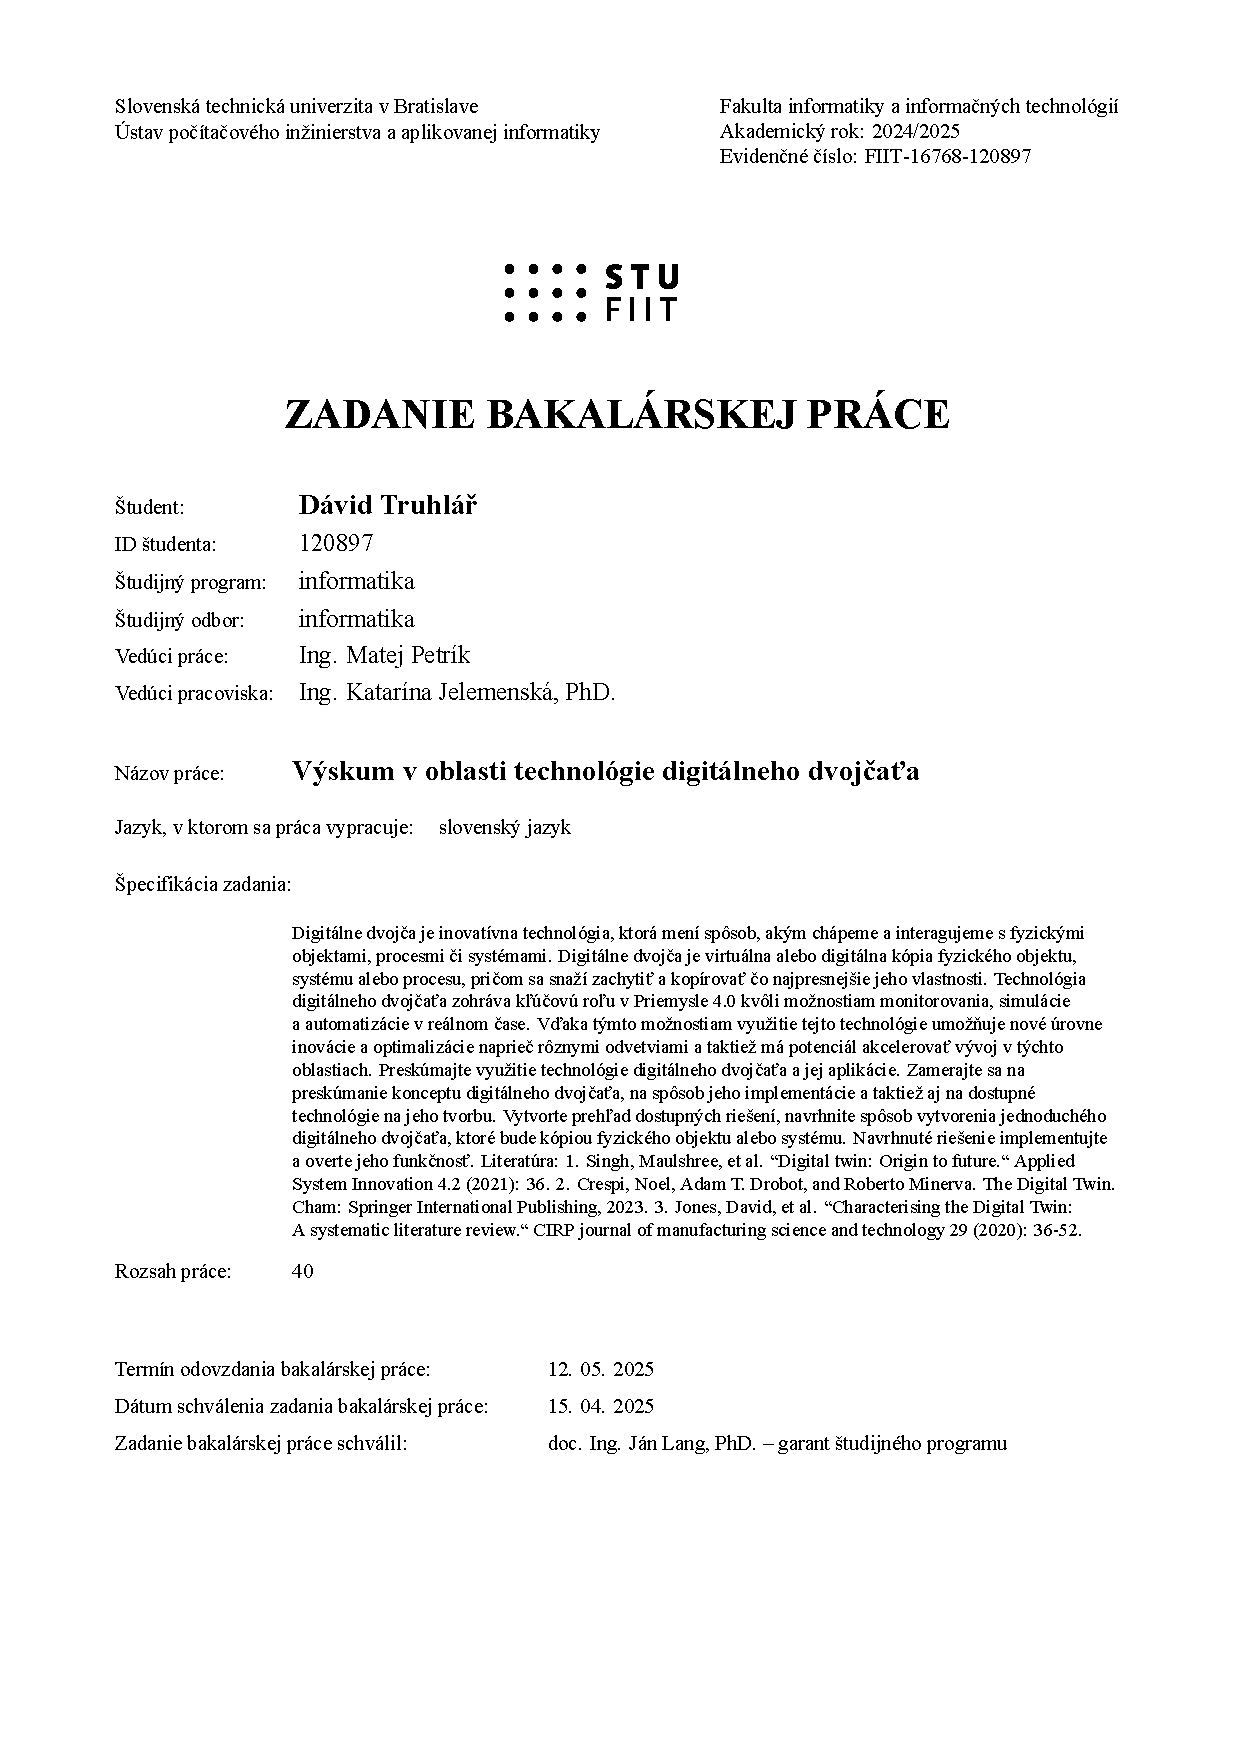
\includepdf[pages=1,scale=0.85]{assets/zadanie.pdf}
\newpage
%\emptypage

% Declaration of honor
\thispagestyle{empty}

\vspace*{\fill}

\ifx\FIITlagEN\undefined
\section*{Čestné prehlásenie}
\else
\section*{Declaration of honor}
\fi
\par{
Čestne vyhlasujem, že som túto prácu vypracoval samostatne, na základe konzultácií a s použitím uvedenej literatúry.
\\ 
\\
}
\ifx\FIITlagEN\undefined
\FIITsignPlaceSK \FIITsignDate
\else
\FIITsignPlace \FIITsignDate
\fi
\hspace*{\fill} \signaturespace{5cm}{\FIITauthor}

\emptypage

% Acknowledgements - Poďakovanie
\thispagestyle{empty}

\vspace*{\fill}

\ifx\FIITlagEN\undefined
\section*{Poďakovanie}
\else
\section*{Acknowledgements}
\fi

Touto cestou by som rád vyjadril úprimné poďakovanie všetkým, ktorí ma podporili a pomohli mi pri vypracovaní tejto bakalárskej práce.

Na prvom mieste patrí moja vďaka školiteľovi Ing. Matejovi Petríkovi za jeho odborné vedenie, ochotu, cenné rady a usmernenia, ktoré výrazne prispeli k realizácii tejto práce. Ďalej vyjadrujem poďakovanie Ing. Matejovi Janebovi za jeho čas a technické konzultácie v oblasti 5G technológií.

Osobitné poďakovanie patrí aj mojej rodine za prejavenú dôveru, trpezlivosť a neustálu podporu počas celého štúdia.

\emptypage

% Annotation
% \include{pages/annotation}

% Table of contents
\ifx\FIITlagEN\undefined
\renewcommand{\contentsname}{Obsah}
\else
\renewcommand{\contentsname}{Table of contents}
\fi
\tableofcontents{}
\emptypage

% List of figures - Zoznam obrázkov
\listoffigures
\emptypage

% List of tables
\listoftables
\emptypage

% List of abbreviations
\thispagestyle{plain}

\ifx\FIITlagEN\undefined
\section*{\Huge Zoznam použitých skratiek}
\markboth{Zoznam použitých skratiek}{Zoznam použitých skratiek}
\else
\section*{\Huge List of abbreviations used}
\markboth{List of abbreviations used}{List of abbreviations used}
\fi
\vskip 1cm

\begin{tabular}{ >{\bfseries}m{2cm} m{10cm} }
AMF     & Funkcia riadenia prístupu a mobility (Access and Mobility Management Function) \\  
AUSF    & Funkcia autentifikačného servera (Authentication Server Function) \\  
BP      & Bakalárska práca \\  
DT      & Digitálne dvojča (Digital Twin) \\  
GDPR    & Všeobecné nariadenie o ochrane údajov (General Data Protection Regulation) \\  
gNB     & Node B novej generácie (Next Generation Node B) \\  
IoT     & Internet vecí (Internet of Things) \\  
IT      & Informačné technológie \\  
ML      & Strojové učenie (Machine Learning) \\  
PCF     & Funkcia politiky a účtovania (Policy and Charging Function) \\  
RAN     & Rádiová prístupová sieť (Radio Access Network) \\  
SMF     & Funkcia riadenia relácií (Session Management Function) \\  
UDM     & Jednotná správa údajov (Unified Data Management) \\  
UDR     & Jednotné úložisko údajov (Unified Data Repository) \\  
UE      & Užívateľské zariadenie (User Equipment) \\  
UPF     & Funkcia používateľskej roviny (User Plane Function) \\  
\end{tabular}

\emptypage

% Enable page numbering
\pagenumbering{arabic}

% Begin refferences segment
\begin{refsegment}

%Technický abstrakt je stručný súhrn práce, obvykle obsahujúci okolo 250 slov. Môže byť štruktúrovaný (napr. obsahovať časti ako účel, metódy, výsledky a záver) alebo neštruktúrovaný. Cieľom je, aby sa študent naučil vytvárať stručné technické zhrnutie svojej práce. {\btHL ½ strany}

\chapter{Technický abstrakt}

5G siete predstavujú základ infraštruktúry pre kritické aplikácie s vysokými nárokmi na nízku latenciu a vysokú spoľahlivosť. V tomto kontexte môžu zohrávaať digitálne dvojčatá (Digital Twin) kľúčovú úlohu pri simulácii, monitorovaní a optimalizácii siete v reálnom čase. Cieľom tejto práce je navrhnúť a implementovať klasifikačný systém využívajúci digitálne dvojča 5G siete, ktorý je schopný v reálnom čase identifikovať typ sieťovej prevádzky (Use Case - UC) pomocou metód strojového učenia.

Navrhnutý systém využíva nástroje Open5GS a UERANSIM na generovanie syntetických metrických dát zo šiestich typov sieťovej záťaže, pričom tieto scenáre pokrývajú ako bežné, tak aj anomálne správanie používateľov. Súčasne prebieha zber dát z reálnej siete a porovnanie rozložení metrík pomocou metód ako KL-divergencia a PCA vizualizácie. Po analýze prieniku medzi syntetickým a reálnym priestorom bol navrhnutý robustný výber metrík pomocou kombinácie Random Forest, RFE, SFS a permutačnej importance.

Výsledný model využíva LSTM architektúru optimalizovanú pomocou Batch normalizácie pre klasifikovanie stavu siete v reálnom čaase. Model trénovaný výhradne na syntetických dátach dosiahol na reálnych dátach presnosť ~13\%, ktorá bola následne zlepšená pomocou online fine-tuningu založeného na správne označených UC hodnotách až na ~50\%. Model je nasadený v Docker kontejneroch, načítava real-time metriky a predikcie sú exportované do Prometheus ako vlastné metriky. Celý systém je vizualizovaný v Grafane, vrátane dôveryhodnosti predikcie a verziovania modelu. 

Práca potvrdzuje, že pri dôslednej doménovej analýze je možné trénovať použiteľný model výhradne na syntetických dátach a následne ho adaptovať na produkčné nasadenie v reálnej 5G infraštruktúre.


\chapter{Laický abstrakt}

\par{
%Laický abstrakt je stručné vysvetlenie výskumnej práce napísané jednoduchým, netechnickým jazykom. Účelom je preukázať plynulosť študenta v komunikačných zručnostiach voči širokej verejnosti zrozumiteľne. Laický abstrakt by mal mať maximálne 250 slov a je neštruktúrovaný. \btHL1/2 strany

Digitálne dvojča predstavuje virtuálny model reálneho systému, ktorý umožňuje sledovať a analyzovať jeho správanie v reálnom čase. V posledných rokoch si táto technológia našla uplatnenie v priemysle, doprave či zdravotníctve. V tejto práci sa venujem vytvoreniu digitálneho dvojčaťa pre 5G sieť s cieľom porozumieť, ako sa správa pri rôznych používateľských scenároch.

Pomocou voľne dostupných nástrojov som vytvoril softvérové prostredie, ktoré simuluje správanie reálnej mobilnej siete. Následne som zbieral dáta nielen zo simulácií, ale aj z reálnych zariadení pripojených do 5G siete. Tieto údaje zahŕňali napríklad počet pripojených používateľov či objem prenesených dát.

Hlavným cieľom bolo overiť, či je možné natrénovať model umelej inteligencie na simulovaných dátach a použiť ho na rozpoznávanie situácií v reálnej sieti. Takýto prístup je bezpečný, flexibilný a umožňuje testovanie aj zriedkavých alebo extrémnych scenárov bez zásahu do reálnej prevádzky.

Výsledný systém dokáže klasifikovať správanie siete podľa typických vzorcov a vytvára priestor pre budúce nasadenie monitorovania a správy sietí. 
}



\thispagestyle{empty}
\chapter{Úvod}

Technológia digitálneho dvojčaťa (DT) predstavuje perspektívny prístup v modernom softvérovom inžinierstve \cite{DimensionOfDTAplication} a telekomunikácií \cite{AplicationsOfDT}. DT umožňuje vytvárať virtuálne kópie fyzických systémov, ktoré v reálnom čase zrkadlia ich správanie pomocou obojsmernej výmeny dát \cite{real_time}. DT nachádzajú praktické uplatnenie v rôznych doménach vrátane výroby \cite{manufacturing}, zdravotníctva \cite{siemens_helthcare} a energetiky, kde umožňujú monitorovanie v reálnom čase, prediktívne riadenie a optimalizáciu procesov \cite{AplicationsOfDT}.

V oblasti sietí, najmä sietí piatej generácie (5G), poskytujú DT nové možnosti v simulácii sieťového správania, včasnej detekcii anomálií a optimalizácii alokácie zdrojov \cite{5gandbeyond}. 5G infraštruktúry sa vyznačujú vysokou heterogenitou, dynamikou a nárokmi na kvalitu služieb (QoS), čo komplikuje ich správu a testovanie \cite{AplicationsOfDT}. DT v tomto kontexte umožňuje testovanie rôznych scenárov vo virtuálnom prostredí bez rizika výpadku služby či narušenia integrity dát. Kľúčovou výzvou pri návrhu DT pre 5G siete je však zabezpečenie dostatočnej vernosti simulácie. Otázna zostáva najmä generalizovateľnosť modelov trénovaných iba na syntetických dátach voči reálnym podmienkam, ktoré sú komplexnejšie a menej predvídateľné. Cieľom tejto práce je preskúmať túto oblasť prostredníctvom návrhu a implementácie jednoduchého DT pre 5G sieť, postaveného na voľne dostupných nástrojoch Open5GS \cite{open5gs} a UERANSIM \cite{ueransim}, a vyhodnotiť schopnosť modelov klasifikovať správanie siete v reálnom čase na základe synteticky generovaných metrík.


\thispagestyle{empty}

\chapter{Formulácia problému a riešenie}

\section{Formulácia problému}
V oblasti 5G sietí predstavujú DT perspektívny nástroj na bezpečné testovanie, monitorovanie a optimalizáciu správania siete. Vysoké nároky 5G na nízku odozvu, spoľahlivosť a flexibilitu riadenia zároveň vyžadujú schopnosť rýchlo identifikovať typické aj neštandardné správanie vrátane anomálií a útokov. Aby bolo možné efektívne trénovať klasifikačné modely bez rizika pre produkčnú infraštruktúru, je nevyhnutné simulovať rôzne scenáre v kontrolovanom prostredí digitálneho dvojčaťa.

Kľúčovým problémom však zostáva otázka, do akej miery môžu modely trénované výhradne na syntetických dátach zo simulovaných prostredí, ako Open5GS a UERANSIM, generalizovať na reálne siete, keďže výrazný nesúlad medzi syntetickými a reálnymi dátami môže obmedziť praktickú využiteľnosť takto vytvorených modelov.

Cieľom tejto bakalárskej práce je preto navrhnúť a implementovať jednoduché DT 5G siete a preskúmať, do akej miery možno synteticky generované metriky využiť na trénovanie modelov schopných klasifikovať správanie v reálnej sieti.

\section{Technický literárny prehľad}
DT predstavuje koncept virtuálnej repliky fyzického objektu alebo systému, ktorá je schopná v reálnom čase odrážať jeho aktuálny stav prostredníctvom obojsmernej výmeny dát (pozri Obr. \ref{fig:PLM}) \cite{DT:OriginToFuture}. Na rozdiel od tradičných modelov alebo simulácií je DT charakteristické dynamickým aktualizovaním svojho správania na základe dát zo sledovaného objektu \cite{systematicReview}. Tento koncept nachádza uplatnenie naprieč viacerými odvetviami vrátane výroby, zdravotníctva, dopravy či energetiky \cite{5gandbeyond}.\\

\begin{figure}[H]
    \centering
    \includegraphics[width=0.8\linewidth]{assets/images/Grieves_PLM_model.png}
    \caption[Model zrkadlených priestorov]{Model zrkadlených priestorov (Mirrored Spaces Model) tak, ako ho vo svojej práci navrhol Grieves \cite{Grieves}. Tento model sa skladá z troch komponentov - reálny priestor (Real Space), virtuálny priestor (Virtual space) a spájací mechanizmus (Linking Mechanism) \cite{DT:OriginToFuture}, ktorý prúdi automatizovane oboma smermi medzi týmito priestormi. Virtuálny priestor vytvára digitálnu reprezentáciu reálnych objektov a podporuje viacero virtuálnych systémov na analýzu, simuláciu alebo predikciu správania fyzických objektov.}
    \label{fig:PLM}
\end{figure}

Vo  svojom výskume Enders a Hoßbachová \cite{DimensionOfDTAplication} identifikovali sektory, kde je používanie DT najrozšírenejšie. Patria sem výroba \cite{manuf}, letecký priemysel \cite{aircraft}, energetika \cite{energy}, automobilový priemysel \cite{automotive}, námorníctvo \cite{marine}, petrochemický priemysel \cite{oil}, poľnohospodárstvo \cite{agriculture}, zdravotníctvo \cite{health}, verejný sektor \cite{education} a ťažba \cite{mining}.

Taktiež identifikovali tri hlavné využitia DT v týchto oblastiach \cite{AplicationsOfDT}: ovládanie, simulovanie a monitorovanie. To však nepokrýva všetky možnosti a spôsoby využitia. DT dnes nájde uplatnenie aj pri dizajnovaní, validácii, predchádzaní chýb, trénovaní a optimalizácii.

Vývoj digitálnych dvojčiat je podporený množstvom softvérových nástrojov líšiacich sa funkcionalitou a cenou. ANSYS Twin Builder je zameraný na presné fyzikálne modelovanie procesov (mechanika, elektromagnetizmus) a je vhodný pre tvorbu inžinierskych DT, pričom patrí medzi najnákladnejšie riešenia \cite{ansys_twin_builder}. Siemens MindSphere ponúka cloudovú platformu na správu dát a monitoring zariadení v priemyselných aplikáciách, s cenou závislou od rozsahu nasadenia \cite{siemens_mindsphere}. MATLAB a Simulink ponúkajú flexibilnú platformu pre tvorbu digitálnych dvojčiat s dôrazom na simuláciu dynamických systémov, modelovanie riadiacich algoritmov a predikciu správania \cite{mathworks_digital_twin}.
Alternatívou bez licenčných nákladov je vlastná implementácia DT prostredí, kde je možné vytvoriť simulované kópie vybraných častí systému. Napríklad v oblasti 5G možno pomocou Open5GS a UERANSIM zostaviť základné virtuálne repliky siete, ktoré v kombinácii s vhodne naprogramovanými skriptami umožňujú budovanie DT.

Ak sa chceme pozrieť na reálne aplikácie DT, Huawei implementoval DT na monitorovanie výrobných liniek \cite{huawei2020}, zatiaľ čo mestá ako Bristol \cite{Bristol} či Singapur \cite{singapur} používajú DT na efektívne riadenie inteligentných mestských systémov. V týchto scenároch DT umožňuje predikciu zlyhaní, optimalizáciu zdrojov a minimalizáciu prestojov. 

V oblasti telekomunikácií sa koncept DT začína uplatňovať na monitorovanie a optimalizáciu sieťových zdrojov v reálnom čase. 5G siete sú charakteristické vysokými nárokmi na nízku latenciu, spoľahlivosť a dynamické riadenie. DT v tomto prostredí umožňuje simuláciu zmien konfigurácie, predikciu anomálií a podporu rozhodovania bez rizika zásahu do produkčnej infraštruktúry \cite{JONES202036}.

Odborná literatúra zároveň upozorňuje, že jednou z hlavných výziev pre DT v oblasti 5G je zabezpečenie dostatočne realistickej reprezentácie dynamických sieťových podmienok, vrátane mobility používateľov, variability záťaže a správy QoS \cite{theDigTwin}.
Niektoré open-source simulačné nástroje ako Open5GS alebo UERANSIM, umožňujú tvorbu syntetických dát pokrývajúcich štandardné scenáre správania siete \cite{openanduerans}, avšak plné zachytenie komplexity reálnej prevádzky zostáva otvorenou výzvou.

Z týchto poznatkov vyplýva, že ďalší výskum by sa mal sústrediť na rozšírenie simulačných možností, kombinovanie syntetických a reálnych dát a na metodiky validácie modelov v podmienkach, ktoré čo najviac odrážajú reálnu prevádzku 5G sietí.

\section{Prehľad riešenia na vysokej úrovni}

Navrhnuté riešenie pozostáva z modulárneho systému na báze DT, ktorého cieľom je analyzovať a klasifikovať správanie 5G siete v kontrolovanom prostredí. Vytvorené DT simuluje vybrané komponenty reálnej siete a umožňuje generovanie syntetických dát, ich zber, spracovanie a následnú aplikáciu modelov strojového učenia. Architektúra systému bola navrhnutá s dôrazom na rozšíriteľnosť, modularitu a experimentálnu reprodukovateľnosť.

Open5GS je open-source implementácia 5G jadra siete, ktorá slúži ako základná riadiaca infraštruktúra pre prichádzajúce spojenia. V navrhnutom riešení zodpovedá za autentifikáciu zariadení, správu session a prideľovanie IP adries.

UERANSIM je emulátor RAN prístupu, ktorý generuje simulovaných používateľov (UE), ktorí sa pripájajú do siete (pozri Obr. \ref{fig:architecture}) cez definované scénare. Umožňuje flexibilne konfigurovať počet zariadení, typy prevádzky a časovanie spojení.

\begin{figure}[H]
    \centering
    \includegraphics[width=0.75\linewidth]{assets//images/core-ue.png}
    \caption[Architektúra komponentov Open5GS a UERANSIM]{Architektúra jednotlivých komponentov Open5GS a UERANSIM a ich vzájomné prepojenie. Open5GS je rozdelené na riadiacu rovinu a rovinu užívateľských dát a obe tieto roviny sú napojené na gNB, ku ktorým sa môžu pripájať zariadenia.}
    \label{fig:architecture}
\end{figure}

Monitorovacia infraštruktúra pozostáva z nástrojov Prometheus, Grafana, Promtail a logwatcher.py. Prometheus zberá metriky zo siete a systémových zdrojov, ktoré sú vizualizované pomocou Grafany. Logwatcher je vlastný Python skript, ktorý analyzuje logy z Open5GS a exportuje vlastné metriky ako napr. počet aktívnych UE či SUCI identifikátory.

Skripty na simuláciu scenárov (UC) slúžia na spúšťanie preddefinovaných testovacích situácií. Každý UC definuje počet zariadení, objem prenesených dát a časovanie spojení, čím vytvára realistické syntetické zaťaženie siete.

Predspracovanie dát a výber metrík (EDA, preprocessing, feature selection) boli vykonané raz pred trénovaním modelu, s cieľom optimalizovať vstup pre model strojového učenia. Výber metrických premenných bol podporený metódami založenými na rozhodovacích stromoch a permutačnej dôležitosti.

Modely strojového učenia boli implementované pomocou LSTM modelov, ktoré sú vhodné pre sekvenčné dáta. Model bol natrénovaný na syntetických dátach a neskôr testovaný na dátach z reálnej siete.

\begin{figure}[H]
    \centering
    \includegraphics[width=0.95\linewidth]{assets//images/arch2.png}
    \caption{Zariadenia generované pomocou UERANSIM sa pripájajú k jadru siete v Open5GS, ktoré loguje udalosti a vystavuje metriky. Tieto údaje sú zbierané pomocou Promethea a logwatcher.py skriptu. Výstupy sú agregované do datasetu, ktorý sa ďalej spracúva v prostredí Jupyter Notebook. Po spracovaní sa dáta využívajú na trénovanie a testovanie modelov strojového učenia. Vizualizácia metrických údajov prebieha súbežne v Grafane.}
    \label{fig:arch}
\end{figure}

Modularita kontajnerizovaného riešenia založeného na Docker Compose umožňuje jednoduché nasadenie a replikáciu prostredia. Open-source komponenty boli zvolené kvôli dostupnosti a možnosti detailnej konfigurácie siete. Použitie syntetických scenárov poskytuje kontrolu nad testovaným správaním bez rizika ovplyvnenia reálnej prevádzky. LSTM siete boli zvolené vďaka schopnosti modelovať časové závislosti, ktoré sú kľúčové pri klasifikácii sieťového správania. Kombinácia reálneho a syntetického vstupu umožňuje overiť možnosti generalizácie modelov v telekomunikačnom prostredí.
 
\section{Hodnotenie rizík}
Implementácia digitálneho dvojčaťa 5G siete spolu s modelom ML prináša rôzne výzvy, ktoré môžu ovplyvniť presnosť klasifikácie, stabilitu a efektívnosť celého systému. 

Nedostatočná kvalita vstupných dát je jedným z najpravdepodobnejších rizík, ktoré môžu viesť k nesprávnym výsledkom modelu. Chyby v dátach alebo ich nereprezentatívnosť, napríklad pri modeloch sieťovej prevádzky (traffic patterns), môžu narušiť presnosť predpovedí \cite{ML_traffic}. Formou zmiernenia je testovanie na rôznych dátových scenároch a aplikácia metód ako krížová validácia a ladenie hyperparametrov, ktoré minimalizujú riziko chýb spojených s podtrénovaním (underfitting) a pretrénovaním (overfitting) \cite{Nguyen}.

Zber kvalitných dát môže byť problematický, pretože mnohé scenáre je potrebné zachytiť v laboratóriu. Bez dostatočných dát môže model generovať neadekvátne predpovede, ktoré nebudé reprezentovať skutočnosť. Riešením môže byť generovanie syntetických údajov \cite{data_generating} a využitie dostupných datasetov z iných projektov \cite{datasets_telecom}, ktoré môžu čiastočne nahradiť reálne dáta a napomôcť k presnejším predpovediam.

Nezvyčajné scenáre, ako vysoké zaťaženie siete (peak loads), neštandardné správanie používateľov či poveternostné podmienky môžu narušiť schopnosť modelu adaptovať sa \cite{challenges_human_factor}. Ak tieto scenáre neobsahujú trénovacie dáta, model nemusí byť pripravený na takéto situácie. Vzhľadom na čas, ktorý máme na získanie a predspracovanie dát, tento problém nemusí byť vo finálnej implementácií vyriešený dostatočne, a preto jeho vyriešenie vyžaduje ďalšiu prácu a zber dát.

Kompatibilita systémov ako srsRAN, Open5GS, UERANSIM a nástrojov Docker nie je vždy automatizovaná, čo môže ovplyvniť celkovú integráciu práce \cite{challenges_human_factor}. Z tohoto dôvodu je vhodné začínať implementáciu na malých izolovaných komponentoch, za neustáleho testovania. Takéto testovanie, a celkový vývoj DT sú časovo veľmi náročné, čo potvrdili aj autori v \cite{USAirForce}. Tento fakt môže negatívne vplývať na výsledok celej práce, nakoľko čas je jedným z kľúčových faktorov, ktoré majú vplyv na množstvo a kvalitu pozberaných dát určených na trénovanie ML modelu.

Konfigurácia siete môže odhaliť citlivé informácie o 5G infraštruktúre či porušenie GDPR \cite{big-data-problems} pri nechcenom zachytení údajov o používateľoch \cite{challenges-technol}. Únik takýchto dát by ohrozil nielen bezpečnosť projektu, ale aj reálnej siete \cite{Dt_Iot_data_worry_about}. Používanie .env súborov na uchovávanie citlivých premenných a simulovanie siete s fiktívnymi údajmi výrazne znižuje riziko úniku.

\section{Experimentálna reprodukovateľnosť a integrácia}
%Fáza inžinierstva riešení by mala byť vykonávaná s ohľadom na reprodukovateľnosť a systémovú integráciu a študenti by mali podrobne opísať, ako sa tejto otázke venovali. Pokiaľ nie sú špeciálne podmienky, kód, modely a dáta použité pri inžinierstve riešení by mali byť voľne dostupné. Modely strojového učenia by mali byť prezentované tak, aby umožňovali ďalšie využitie bez nutnosti rekvalifikácie. Tam, kde je to možné, použite riešenia v kontajneroch, ktoré zabezpečia použiteľnosť produktu alebo služby aj pri zmene základnej technológie. | 3 strany

Pre zabezpečenie experimentálnej reprodukovateľnosti a jednoduchej integrácie bola zvolená kontajnerizovaná architektúra pomocou Docker a Docker Compose. Namiesto vytvárania vlastných konfiguračných súborov a obrazov bol použitý existujúci open-source repozitár \texttt{herlesupreeth/docker\_open5gs} \cite{herlesupreeth}, ktorý poskytuje dockerizované prostredie pre komponenty siete 5G vrátane \textbf{Open5GS}, \textbf{UERANSIM}, ako aj voliteľnej integrácie s \textbf{Prometheus} a \textbf{Grafana} na zber a vizualizáciu metrík.

Repozitár bol naklonovaný z GitHubu a jednotlivé obrazy boli zostavené pomocou príkazov:


Niektoré súbory z originálnej implementácie boli upravené pre potreby tohoto projektu. Do yaml súboru, ktorým sa spúšťali niektoré komponenty boli pridané ďalšie služby tak, aby stačil jeden príkaz pre spustenie všetkých komponentov.

Do súboru \textbf{deploy-all.yaml} bola pridaná služba pre integráciu služby NetData \cite{netdata}. Najskôr bolo treba sa na službe zaregistrovať a vytvoriť pracovný priestor. NetData následne ponúka možnosť použiť ich API priamo pomocou Dockeru. 

Spustenie kontajnerov bolo upravené tak, aby sa dalo spúšťať všetko jedným príkazom:

\begin{lstlisting}[language=bash,caption={Build pre jednotlivé docker images}, style=bashstyle]
docker compose -f deploy-all.yaml up --build -d
\end{lstlisting}

Táto voľba bola motivovaná cieľom maximalizovať znovupoužiteľnosť a minimalizovať konfiguračné chyby. Repozitár je aktívne udržiavaný a poskytuje konzistentné a overené nastavenia, ktoré výrazne urýchľujú vývojový proces. Hlavnou výhodou tohto prístupu je zníženie bariéry pre reprodukovateľnosť – akýkoľvek výskumník s podporovaným operačným systémom a Dockerom môže systém replikovať lokálne v priebehu niekoľkých minút. Nevýhodou je menšia kontrola nad interným nastavením kontajnerov, čo môže byť limitujúce pri pokročilejších úpravách.

Pre účely monitorovania spotreby systémových zdrojov bola do architektúry doplnená open-source platforma \textbf{NetData}. Táto služba bola nainštalovaná priamo do Docker hosta a nakonfigurovaná na sledovanie jednotlivých kontajnerov cez dostupné Docker plug-iny. NetData poskytuje prehľad o využití \textbf{RAM}, \textbf{CPU}, \textbf{siete}, ako aj o \textbf{sieťovej komunikácii jednotlivých kontajnerov}, čo je kľúčové pre ladanie a optimalizáciu simulácií. 

Monitorovanie pomocou NetData zvyšuje transparentnosť experimentálneho prostredia a umožňuje identifikovať úzke miesta pri spustení viacerých UEs alebo vysokom trafficu. Zároveň je vďaka tomu možné porovnávať výkonnostné profily experimentov medzi rôznymi behmi, čo je kľúčovým predpokladom pre experimentálnu reprodukovateľnosť.

\section{Udržateľnosť a environmentálny dopad}
DT predstavujú účinný nástroj na optimalizáciu prevádzkových procesov – v porovnaní s fyzickým testovaním umožňujú výrazne znížiť spotrebu zdrojov, produkciu odpadu aj operačné riziká \cite{enviro_raw_materials}. V kontexte návrhu DT 5G siete, implementovaného v rámci tejto práce, bola environmentálna udržateľnosť reflektovaná v niekoľkých rovinách.

Z pohľadu výpočtovej náročnosti bola celá infraštruktúra navrhnutá s cieľom minimalizovať energetickú záťaž. Celý systém bol prevádzkovaný na lokálnom výpočtovom zariadení bez využitia centralizovaných cloudových služieb či grafických akcelerátorov (GPU). Kombinácia kontajnerizovaných služieb (Docker Compose) a voľne dostupných softvérových nástrojov (Open5GS, UERANSIM, Prometheus, Grafana) umožnila zabezpečiť nízku spotrebu zdrojov \cite{docker_enviro} pri zachovaní dostatočnej funkcionality pre experimentálne overenie konceptu \cite{docker_enviro_2}.

V širšom zmysle sú DT považované za technológiu s potenciálom znižovať uhlíkovú stopu prostredníctvom presnejšej správy sietí, prediktívnej údržby a minimalizácie potreby fyzických zásahov do infraštruktúry \cite{DT_edge_networks_IoT, enviro}. Aj keď prediktívne modelovanie nebolo predmetom tejto práce, implementovaný systém poskytuje základ, na ktorom je možné budovať systémy podporujúce rozhodovanie s pozitívnym environmentálnym dopadom \cite{malaysia_enviro}.

Navyše, architektúra riešenia je modularizovaná, čo umožňuje selektívnu údržbu a výmenu komponentov bez nutnosti reinštalácie celého systému. Tento návrhový prístup je zároveň v súlade s princípmi zeleného softvérového inžinierstva, ktoré zdôrazňujú energetickú efektivitu a podporujú dlhodobú udržateľnosť softvérových riešení \cite{modular_sw}.

Navrhnutý systém teda nielen zohľadňuje technologickú efektivitu a experimentálnu hodnotu, ale zároveň reflektuje environmentálne požiadavky pri návrhu a testovaní moderných komunikačných systémov.

\section{Zamestnateľnosť}
Táto bakalárska práca, zameraná na rozvoj teoretických znalostí v oblasti digitálnych dvojčiat v spojení s praktickou implementáciou a optimalizáciou 5G sietí, vedie k rozšíreniu zručností vo viacerých kľúčových oblastiach technologického sektora. V neposlednom rade strojové učenie, použité na predikciu správania implementovaného digitálneho dvojčaťa, zasahuje aj do oblasti dátovej vedy.

Vďaka formátu práce autori prejdú celým cyklom realizácie projektu, od prieskumu technológií cez návrh až po implementáciu a testovanie. Týmto získajú ucelený a komplexný pohľad na vývoj a riadenie softvérových projektov, ako aj na plánovanie, organizáciu a efektívnu komunikáciu.

Takáto kombinácia technických, projektových a komunikačných schopností môže významne zvýšiť hodnotu autorov na trhu práce, najmä v budúcnosti, keďže problematika digitálnych dvojčiat a 5G sietí je stále viac žiadaná a nachádza uplatnenie v rôznych odvetviach.

\section{Tímová práca, diverzita a inklúzia}
%\par{
%Ak sa na projekte podieľajú odborníci z viacerých odborov, študent by mal implementovať procesy a opísať techniky pre zdieľanie úloh a (pochopenie) znalostí medzi rôznymi stranami. Mali by sa opísať problémy a stratégie na ich zmiernenie, aby sa zabezpečilo dokončenie projektu v stanovenom časovom harmonograme. Táto časť by mala obsahovať aj úvahy o diverzite a inklúzii. | ½-1 strana
%}
\par{
Teamwork and Knowledge Sharing: \\
- spolupráca s Matejom a Matejom

Diversity and Inclusion:
- Ageism - pomoc pre všetky vekové skupiny?
- Disabled people? hearing, vision ...
- môže im to DT nejko pomôcť?
- Prehľadná dokumentáia a návod pre možnú spoloprácu...
}

Spolupráca s konzultantom a inými odborníkmi: Môžete zdôrazniť, ako ste spolupracovali s konzultantom, odborníkmi alebo kolegami, aby ste získali spätnú väzbu alebo konzultovali technické aspekty projektu.

Diverzia myšlienok a prístupov: Aj keď ste projekt riešili individuálne, môžete opísať, ako ste zohľadnili rôzne perspektívy pri výbere riešení a metodík. Napríklad môžete zdôrazniť, že ste čerpali z rôznych zdrojov, ako sú články, výskumy a prípadové štúdie, aby ste vytvorili univerzálne použiteľný a inkluzívny návrh.

Prístupnosť a inklúzia výsledkov projektu: Opíšte, ako váš projekt môže byť prínosný pre širšiu komunitu používateľov. Napríklad, ak je váš digitálny dvojča schopné zlepšiť efektivitu nasadzovania 5G sietí, môže byť relevantný aj pre menej rozvinuté regióny alebo oblasti so zníženými zdrojmi.

Schopnosť prispôsobiť projekt tímovému pracovnému prostrediu: Môžete uviesť, že ste navrhli systém s ohľadom na modularitu a jednoduchú integráciu, čo umožňuje budúcu spoluprácu tímov na rozšírení projektu


\chapter{Záver}

V rámci tejto bakalárskej práce bol navrhnutý a implementovaný základný model digitálneho dvojčaťa (DT) pre 5G sieť, ktorý umožňuje simuláciu správania siete a zber dát z fyzickej i simulovanej infraštruktúry. Použitím nástrojov Open5GS a UERANSIM bol vytvorený kontrolovaný experimentálny priestor, v ktorom bolo možné testovať rôzne používateľské scenáre bez zásahu do reálnej siete. Výsledky však ukazujú, že samotné Open5GS metriky zo simulovaného prostredia nie sú postačujúce na vytvorenie klasifikačného modelu, ktorý by spoľahlivo identifikoval správanie v reálnej 5G sieti. Modely trénované výhradne na syntetických dátach dosahovali výrazne horšiu presnosť pri testovaní na reálnych dátach (~16\%), čo poukazuje na značné rozdiely medzi simulovaným a skutočným sieťovým správaním. Táto skutočnosť zároveň poukazuje na potrebu pokročilejších metód prepojenia medzi syntetickými a reálnymi dátami.

Tieto zistenia poukazujú na viaceré limity implementovaného prístupu, ktoré je potrebné otvorene pomenovať. V prvom rade sa ukázalo, že syntetické metriky generované pomocou Open5GS majú obmedzenú schopnosť zachytiť komplexitu reálneho sieťového správania. Chýba im detailná reprezentácia QoS mechanizmov, realistický prenos na aplikačnej vrstve, ako aj podpora mobility, čo výrazne znižuje použiteľnosť týchto simulácií ako základ pre trénovanie modelov s dobrou generalizačnou schopnosťou. Hoci boli testované viaceré architektúry klasifikačných modelov (vrátane attention mechanizmu a batch normalizácie), výkonnosť na reálnych dátach ostávala nízka, čo naznačuje, že problém spočíva predovšetkým v obmedzenej kvalite dát. Navyše, použité metriky sa týkali výlučne core vrstvy, pričom chýbali detailnejšie údaje z RAN vrstvy, ako napríklad parametre rádiového signálu alebo využitie fyzických kanálov. Z pohľadu reálneho experimentálneho zberu bola práca obmedzená na malý počet zariadení, krátke trvanie meraní, čo mohlo ovplyvniť robustnosť výstupov. Hoci väčšina simulácií reprezentovala štandardné prípady správania, v jednom z prípadov bol zaradený aj anomálny scenár s odmietnutím pripojenia na základe neplatného IMSI, čo čiastočne zvýšilo rozmanitosť dát.

Výsledky tejto práce naznačujú, že DT môžu mať významné uplatnenie v oblasti riadenia a optimalizácie 5G sietí, predovšetkým ako nástroj na bezpečné testovanie sieťových zmien, včasné odhaľovanie anomálií a trénovanie systémov umelej inteligencie mimo produkčného prostredia. Do budúcnosti by mal byť výskum orientovaný na zvýšenie vernosti simulácií a zlepšenie kvality dát použitých na trénovanie modelov. Za účelom premostenia medzi syntetickými a reálnymi dátami sa ako perspektívna javí kombinácia metrických údajov z Open5GS s dátami zachytenými v podobe paketov (PCAP), čo umožní extrahovať dotatočné charakteristiky sieťového správania a vrstviť informácie naprieč L2–L7. Zároveň je potrebné preskúmať možnosti aplikácie pokročilých doménovo adaptačných techník, ktoré by mohli znížiť závislosť na rozsiahlych reálnych datasetoch.

Práca ukazuje, že real-time klasifikácia a online trénovanie modelov je technicky realizovateľné v rámci DT, hoci zatiaľ len pri použití syntetických dát. Výzvou do budúcnosti ostáva rozšíriť tento prístup aj na reálne sieťové prostredie a uzavrieť spätnú regulačnú slučku — teda umožniť systému nielen detegovať anomálie v reálnom čase, ale aj automaticky reagovať vhodnou rekonfiguráciou siete alebo notifikáciou správcu. Takýto obojsmerný tok dát medzi fyzickým a digitálnym prostredím predstavuje ďalší krok k autonómnym, adaptívnym sieťam piatej generácie. 
%\emptypage

\begin{comment}
\ifx\FIITlagEN\undefined
\else
\include{pages/resume}
\fi
\end{comment}

% Bibliography
\thispagestyle{empty}
\printbibliography[heading=references,segment=\therefsegment]

% no page numbers for appendicies
\addtocontents{toc}{\protect\setcounter{tocdepth}{0}}
\addtocontents{toc}{\cftpagenumbersoff{chapter}}

%\emptypage

\end{refsegment}

% Appendix
\appendix

% Time schedule
\thispagestyle{empty}

\ifx\FIITlagEN\undefined
\chapter{Harmonogram práce}
\else
\chapter{Project task schedule}
\fi

\pagenumbering{arabic}
\renewcommand*{\thepage}{A-\arabic{page}}

\section{Zimný semester}

\begin{tabular}{|p{2.7cm}||p{10.4cm}|}
\hline
1. - 5. týždeň    & Konzultácie, rešerš problematiky  \\
\hline
6. týždeň    & Formulácia problému \\
\hline
7. týždeň   & Technický literárny prehľad \\
\hline
8. týždeň                       & Konzultovanie, Zamestnateľnosť   \\
\hline
9. - 10. týždeň   & Implementovanie pripomenutých zmien,  Hodnotenie rizík, Udržateľnosť a environmentálny dopad  \\
\hline
11. týždeň  & Návrh riešenia na vysokej úrovni \\
\hline
12. týždeň & Úvod, Konzultovanie, Odovzdávanie BP 1 \\
\hline
\end{tabular}

\subsection{Vyjadrenie k harmonogramu}
Harmonogram sa dodržal, čo prispelo k systematickému postupu pri spracovaní BP. Pravidelné konzultácie s vedúcim práce zohrali kľúčovú úlohu pri jej realizácii. Vedúci poskytoval pripomienky a odporúčania, na základe ktorých sa jednotlivé časti práce mohli upraviť do súčasnej podoby. Tento proces mi umožnil efektívne riešiť prípadné nedostatky a zabezpečiť súčasnú kvalitu výsledného dokumentu.


\section{Letný semester}

\begin{tabular}{|p{2.7cm}||p{6.2cm}||p{4.2cm}|}
\hline
Týždeň & Bakalárska práca & Článok \\
\hline
1. - 2. týždeň & Tímová práca, diverzita a inklúzia & Súvisiaca práca  \\
\hline
3. - 4. týždeň & Open5GS, UERANSIM, Zber dát & Úvod, Metodológia, Kľúčové slová \\
\hline
5. - 7.  týždeň  & Zber dát, Štúdium LSTM & Opis Modelu  \\
\hline
8. - 10. týždeň & ML model, trénovanie, Reprodukovateľnosť a integrácia & Evaluácia a Diskusia   \\
\hline
11. týždeň & Technický abstrakt, laický abstrakt & Záver, Abstrakt  \\
\hline
12. týždeň &  Zhrnutie, úpravy, konzultovanie & Budúci výskum \\
\hline
\end{tabular}

\subsection{Vyjadrenie k harmonogramu}
Harmonogram sa vo všeobecnosti podarilo dodržať, hoci práca na niektorých úlohách bola náročnejšia, než sa pôvodne očakávalo. Najmä zber dát a implementácia riešenia si vyžadovali viac času a experimentovania. Vďaka systematickému postupu, pravidelnej práci a priebežným konzultáciám sa však podarilo udržať plánovaný smer a postupne napredovať. Tento prístup umožnil priebežné identifikovanie problémov, ich efektívne riešenie a priebežné zlepšovanie kvality výstupov, čo sa pozitívne prejavilo aj na výslednom spracovaní bakalárskej práce a sprievodného článku.

\setcounter{figure}{0}
\setcounter{listing}{0}

\chapter{Používateľská príručka}
\label{appendix:userguide}
\pagenumbering{arabic}
\renewcommand*{\thepage}{B-\arabic{page}}

\begin{refsegment}

\section*{Používateľská príručka}

\subsection*{Platformy a kompatibilita}
\begin{itemize}
  \item macOS Sequoia 15.4
  \item Ubuntu 22.04.3 LTS
  \item Windows 11 Home s nainštalovaným WSL2
\end{itemize}

\subsection*{Požiadavky}
Git (verzia 2.39.5), Docker (verzia 28.0.1)


\subsection*{Inštalácia a spustenie systému}
\begin{enumerate}
  \item Klonujte repozitár a prejdite do adresára projektu:
  \begin{verbatim}
  git clone https://github.com/xtruhlar/5GDigitalTwin.git
  cd 5GDigitalTwin/Implementation
  \end{verbatim}

  \item Vytvorte Docker obrazy:
  \begin{verbatim}
  cd ./base
  docker build -t docker_open5gs .

  cd ../ueransim
  docker build -t docker_ueransim .

  cd ..
  \end{verbatim}

  \item Nastavte premenné prostredia:
  \begin{verbatim}
  cp .env.example .env

  set -a
  source .env
  set +a
  \end{verbatim}

  \item Spustite celý systém pomocou Docker Compose:
  \begin{verbatim}
  docker compose -f deploy-all.yaml up --build -d
  \end{verbatim}

  \item Naimportujte preddefinovaných účastníkov do MongoDB:
  \begin{verbatim}
  docker exec -it mongo mkdir -p /data/backup
  docker cp ./mongodb_backup/open5gs mongo:/data/backup/open5gs
  docker exec -it mongo mongorestore \ 
    --uri="mongodb://localhost:27017" \
    --db open5gs /data/backup/open5gs
  \end{verbatim}

  \item Overte funkčnosť jadra siete cez Open5GS WebUI: \\ 
  Otvorte \url{http://localhost:9999}  
  Prihlásenie: \\ Meno: \texttt{admin} \\ Heslo: \texttt{1423}

  \item Spustite UERANSIM gNB:
  \begin{verbatim}
  docker compose -f nr-gnb.yaml -p gnodeb up -d && \
    docker container attach nr_gnb
  \end{verbatim}

  \item Pripojte registrované zariadenie (UE):
  \begin{verbatim}
  docker compose -f nr-UEs/nr-ue1.yaml -p ues up --build -d
  \end{verbatim}

  \item Vizualizácia klasifikovaného stavu 5G siete:  
  Otvorte Grafanu na \url{http://localhost:3000}  
  Prihlásenie:\\ Meno: \texttt{open5gs} \\ Heslo: \texttt{open5gs}  
  \\Potom kliknite na \texttt{Dashboards → Current state Dash}
\end{enumerate}

% Bibliography
\printbibliography[heading=referencessec,segment=\therefsegment,resetnumbers=true]

\end{refsegment}

% Contents of the digital medium
\thispagestyle{empty}

\ifx\FIITlagEN\undefined
\chapter{Obsah digitálneho média}
\else
\chapter{Contents of the digital medium}
\fi

\pagenumbering{arabic}
\renewcommand*{\thepage}{C-\arabic{page}}

\ifx\FIITlagEN\undefined
\par Evidenčné číslo práce v informačnom systéme: \FIITevidenceNumber
\else
\par Registration number of the thesis in the information system: \FIITevidenceNumber
\fi

\ifx\FIITlagEN\undefined
\par Obsah digitálnej časti práce (archív ZIP):
\else
\par Contents of the digital medium (ZIP archive):
\fi

\begin{minted}[linenos=false]{text}
Zložka                      Obsah
/data                       Datasety, Jupyter notebooky, a LSTM modely
    /backup                 Pravidelné ukladanie dát
    /datasets               Datasety syntetických a reálnych dát
    /Jupyter Notebooks Output       HTML súbory
    /logs_real_5G           Zložka s log súbormy z reálnej 5G siete
    /Model                  Modely, konfigurácie, škálovače a predspracované dáta
        /json               Konfiguračné súbory pre modely
        /preprocessed_data
        /scaler
        /trained_models     Modely uložené po trénovaní
    current_uc.txt          Aktuálny UC podľa bežiaceho skriptu
    log_execution.log
    main.ipynb              Notebook, ktorý zberá metriky, spája ich s logmi a UC
    running_data.csv        Data za poslednú minútu
/log                        Logy zo sieťových funkcií
    amf.log
    ausf.log
    bsf.log
    nrf.log
    nssf.log
    pcf.log
    scp.log
    smf.log
    udm.log
    udr.log
    upf.log
/loki                       Spojenie logov a Grafany pomocou Loki
    loki-config.yaml
/nr-UEs                     Konfiguračné súbory pre UE
/open5gs                    Open5GS
    /amf                    Konfigurácia AMF
        amf_init.sh
        amf.yaml
    /ausf                   Konfigurácia AUSF
        ausf_init.sh
        ausf.yaml
    /base                   Dockerfile pre Open5GS, WebUI a MongoDB
        Dockerfile
        open5gs_init.sh
    /bsf                    Konfigurácia BSF
        bsf_init.sh
        bsf.yaml
    /grafana                Konfigurácia Grafany, Dashboard, Zdroje
        /dashboards         Dashboard
            current_state.json
            current_state.yaml
        /datasources
            loki.yaml
            prometheus_open5gs.yaml
    /metrics                Konfigurácia Prometheusa, Dockerfile
        Dockerfile
        metrics_init.sh
        prometheus.yaml
    /mongodb_backup         Uložené DB s registrovanými UE
        /open5gs            DB
            accounts.bson
            accounts.metadata.json
            sessions.bson
            sessions.metadata.json
            subscribers.bson
            subscribers.metadata.json
    /nrf                    Konfigurácia NRF
        nrf_init.sh
        nrf.yaml
    /nssf                   Konfigurácia NSSF
        nssf_init.sh
        nssf.yaml
    /pcf                    Konfigurácia PCF
        pcf_init.sh
        pcf.yaml
    /scp                    Konfigurácia SCP
        scp_init.sh
        scp.yaml
    /smf                    Konfigurácia SMF
        ip_utils.py
        make_certs.sh
        smf_4g.yaml
        smf_init.sh
        smf.conf
        smf.yaml
    /udm                    Konfigurácia UDM
        curve25519-1.key
        secp256r1-2.key
        udm_init.sh
        udm.yaml
    /udr                    Konfigurácia UDR
        udr_init.sh
        udr.yaml
    /upf                    Konfigurácia UPF
        ip_utils.py
        tun_if.py
        upf_init.sh
        upf.yaml
    /webui                  Konfigurácia WebUI
        webui_init.sh
/promtail                   Konfigurácia Promtail
    promtail-config.yaml
/ueransim                   Konfigurácia UERANSIM, UE súbory, Dockerfile
    /init_scripts           UE skripty
    /yaml_configs           UE konfigurácie
    Dockerfile
    ueransim_image_init.sh
    ueransim_gnb_init.sh
    ueransim_gnb.yaml
.env.example                Premenné prostredia
deploy-all.yaml             Hlavný yaml pre Docker compose
Dockerfile.networkwatcher   Dockerfile pre skript sledujúci aktuálny stav siete
network_watcher.py          Skript - Aktuálny stav, klasifikácia, fine-tunning
nr-gnb.yaml                 Konfiguračný súbor pre gNodeB
running_network.py          Skript, ktorý náhodne spúšta UC{1 - 6}
uc1.py
uc2.py
uc3.py
uc4.py
uc5.py
uc6.py

\end{minted}

% only if digital medium contents exceed 1 GB
% \par Digitálna časť práce má veľkosť 3.75 GB, kvôli čomu je uložená v systéme G Suite for Education.


\ifx\FIITlagEN\undefined
\par Názov odovzdaného archívu: \FIITArchiveName.
\else
\par Name of the submitted archive: \FIITArchiveName.
\fi


% Contents of the digital medium
\thispagestyle{empty}

\pagenumbering{arabic}
\renewcommand*{\thepage}{D-\arabic{page}}

\ifx\FIITlagEN\undefined
\chapter{Technická dokumentácia}
\else
\chapter{Technical documentation}
\fi

\vspace{1em}
\noindent
Táto kapitola obsahuje podrobnú technickú dokumentáciu projektu Digital Twin of 5G Network. Obsah dokumentu bol vytvorený automaticky pomocou nástroja \texttt{Sphinx} a slúži ako referenčný manuál pre používateľov a vývojárov. Dokumentácia je vyhotovená v anglickom jazyku, keďže projekt využíva množstvo externých knižníc, nástrojov a terminológie, ktorá je bežne dostupná v angličtine. Zároveň to uľahčuje prípadnú integráciu projektu do medzinárodného výskumu či tímovej spolupráce. Okrem samotnej dokumentácie dokoženej v tejto prílohe, sa technická dokumentácia nachádza aj na webstránke\footnote{\url{https://xtruhlar.github.io/5GDigitalTwin/}} repozitára tohoto projektu. 

% Vloženie PDF od 2. strany
\newcounter{docpage}
\setcounter{docpage}{1}

\includepdf[
  pages=2-27,
  scale=0.85,
  pagecommand={\thispagestyle{fancy}\renewcommand*{\thepage}{D-\arabic{page}}}
]{assets/Technická dokumentácia.pdf}





\emptypage

\end{document}
